\subsection{Old systems}
\subsubsection{Shift / Caesar}
Key $K \in \mathbb{Z}_{26}$
\[ e_k(m_i) =  m_i + k \mod 26 \]
\[ d_k(c_i) = c_i - k \mod 26 \]

\subsubsection{Affine}
Key $K = (a \times b) \in (\mathbb{Z}_{26}^* \times \mathbb{Z}_{26}$)

\[ e_k(m_i) = a \cdot m_i + k \mod 26 \]
\[ d_k(c_i) = a^{-1}(c_i - b) \mod 26 \]

$a$ must have a multiplicative inverse ($a^{-1}$)

\subsubsection{Vigenere}
\[ e_k (m) = (m_0 + k_0, m_1 + k_1, \ldots, m_{j-1} + k_{j-1} ) \mod 26 \]
\[ d_k (c) = (c_0 - k_0 , c_1 - k_1 , \ldots, c_{j-1} - k_{j-1} ) \mod 26 \]

Message $m$ is split into blocks of same length as key $k$ if $length(m) > length(k)$

\subsubsection{Hill}
Key is a $j \times j$ \emph{invertible} matrix over $\mathbb{Z}_{26}$. Message $m$ is regarded as vectors of length $j$.

\begin{figure}[H]
\centering
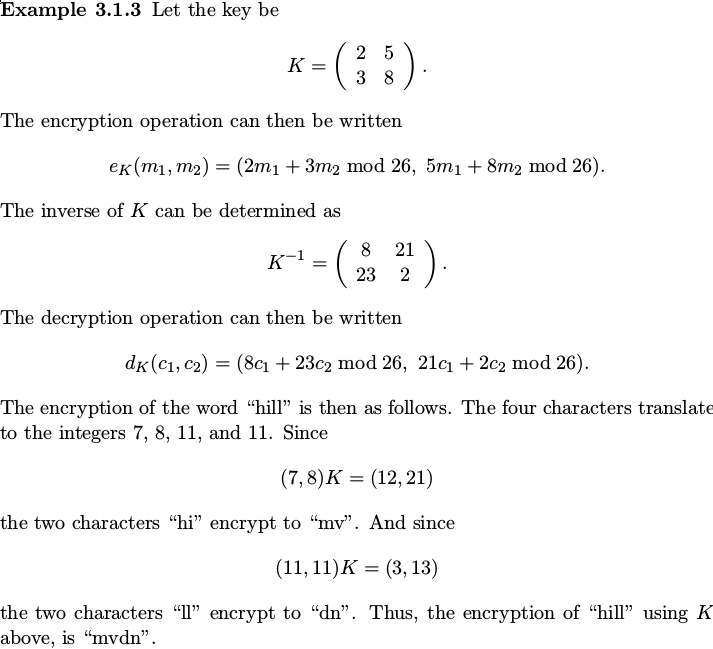
\includegraphics[scale=0.3]{images/1-hill.png}
\caption{Example of Hill cipher enc/dec}
\end{figure}